This section presents the implementation of our three step methodology presented in Section \ref{sec:multiscale-framework}.
We start by describing the methods behind the initial state construction in Section \ref{sec:state-construction-impl}
and then continue to present implementation details of steps two and three in sections \ref{sec:transition-probs-impl}
and \ref{sec:state-aggregation-impl} respectively.

\subsection{Initial State Construction}
\label{sec:state-construction-impl}

As described in section \ref{sec:framework-states} the initial state construction is performed by partitioning
the data points and associating each partition with a single state. The literature suggests many partitioning
algorithms, including those that produce a hierarchical partition. The computational complexity of these algorithms
is, however $O(n^2)$, rendering them unsuitable for large datasets.

To avoid this computational cost, we first create a flat partition of the data space and later aggregate these
partitions to obtain a hierarchical structure.

Following the intuition of Section \ref{sec:framework-states} we consider two data points similar if they lie close
to each other in Euclidean space. \lstopar{Other distance measures are also possible but are out of scope of this paper.}
We use either K-Means or DP-means \cite{DBLP:journals/corr/abs-1111-0352} to construct the partition, representing each 
partition as a Voronoi cell around its centroid. When using StreamStory in real time, the current state is thus
selected by assigning the current sample to the nearest centroid using the following formula:
\begin{equation}
	\nonumber
	i = \argmin_{i \in \mathbb{N}_k} \|x - \mu_i\|.
\end{equation}

We note that the number of centroids (in case of K-Means) or the cluster radius (in case of DP-means) should
be chosen based on domain knowledge and the level of detail users desire. This parameter also effects the 
initial model construction time as demonstrated in Section \ref{sec:implementation}.

\subsection{Modeling Transition Probabilities}
\label{sec:transition-probs-impl}

As described in Section \ref{sec:framework-transitions} we model state transitions using the continuous
time Markov chain framework, first presented in Section \ref{sec:preliminaries}. The transitions are 
modeled on the finest scale and are then aggregated using the formula presented in Section \ref{sec:framework-aggregation}.

We allow users to select a subset of attributes which are used to model transition rates. Since the
jump process from state $i$ to state $j$ can be characterized as a Poisson process, we can model its
transition rate $q_{ij}$ as a function of these attributes $q_{ij} = q_{ij}(x)$. We do this by first
discretizing the continuous time parameter into a discrete sequence $(0, \epsilon, 2\epsilon, ...)$,
estimating the transition rates as
\begin{equation}
	q_{ij}(x) = \frac{\epsilon}{\tilde{p}_{ij}(x)}
\end{equation}
where $\tilde{p}_{ij}$ is the estimated probability of jumping from state $i$ to state $j$ in time
$\epsilon$.

Suppose the process is in state $i$ at time $t$ and define a random variable $J_i = j \Leftrightarrow X_{t + \epsilon} = j$.
$J_i$ then has a multinomial distribution with parameters $(p_{i1}, p_{i1}, ..., p_{in})$ which can be 
modeled using a nominal logistic regression model \cite{glm-introduction} to estimate $\tilde{p}_{ij}(x)$.
The transition rate matrix is then constructed on-the-fly from a matrix of logistic regression models.

\lstopar{
We need to explain why modeling transitions using signals is useful and why it is used.
In previous documents I went on blabbering that by modeling transitions this way, we allow
the possibility of users observing the dynamics in alternate configurations and simulating
what would happen if they changed some parameter. (This was more or less BS though)
}

\subsection{Aggregation}
\label{sec:state-aggregation-impl}

With a fine partition already available, our methodology merges partitions to obtain a hierarchical structure. We employ agglomerative clustering \cite{Murtagh83} producing a hierarchical partition structure. Agglomerative clustering initially treats each partition as a singleton cluster and represents them using a distance matrix $D \in \mathbb{R}^n \times \mathbb{R}^n$ with each element $D_{ij}$ representing the distance between the $i$-th and $j$-th cluster. We note that although the algorithm can be used with any distance metric, we follow the intuition from Section \ref{sec:framework-states} and use Euclidean distance between the state centroids:
\begin{equation}
	\nonumber
	D_{ij} = d(c_i, c_j) = \|c_i - c_j\|_2.
\end{equation}
The algorithm then recursively merges pairs of clusters until only a single cluster remains, producing a cluster tree or \textit{dendrogram}. The partitions chosen for merging are the ones with the minimal entry in the distance matrix $D$:
\begin{equation}
	\nonumber
	(i_{min},j_{min}) = \argmin\limits_{i \neq j}D_{ij}.
\end{equation}
Once the clusters are merged, the entries in the distance matrix that correspond to the merged clusters are updated. This update is called a linkage criteria \lstopar{[cite???]} and determines the distance between clusters as a function of the pairwise distances between their elements. The most popular linkage criteria in the literature are: single-linkage, complete-linkage and average (or mean) linkage. Our experiments show no significant difference between the three and therefore we choose to use the mean linkage criteria:
\begin{equation}
	\nonumber
	D_{S_i,S_j} = \frac{1}{\left|S_i\right|\left|S_j\right|}\sum\limits_{i \in S_i}\sum\limits_{j \in S_j} d(c_i,c_j)
\end{equation}

The distance between the merged clusters $D_{i_{min} j_{min}}$ is used as the $y$ coordinate of the resulting dendrogram, or in our case as the scale where the merged \lstopar{state/cluster} first appears. Figure \ref{fig:dendrogram} shows the relationship between a dendrogram and \lstopar{our visualization}.
\begin{figure}[h!]
	\centering
	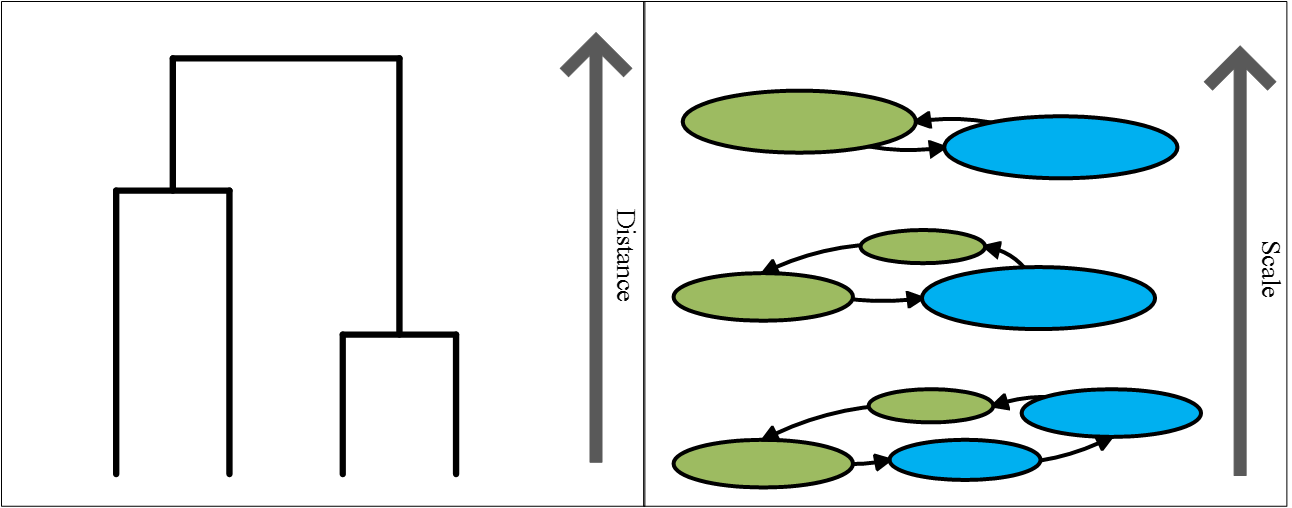
\includegraphics[width=\columnwidth]{dendrogram}
	\caption{\lstopar{TODO}}
	\label{fig:dendrogram}
\end{figure}
The initial finest-scale states are assigned scale $0$. Let $S$ be coarser-scale, aggregated state, aggregating states $A$ and $B$. The scale of $S$ is then defined as:
\begin{equation}
	\nonumber
	s(S) = \frac{1}{\left|A\right|\left|B\right|}\sum\limits_{i \in A}\sum\limits_{j \in B} d(c_i,c_j)
\end{equation} 
